\documentclass[conference]{IEEEtran}

% *** GRAPHICS RELATED PACKAGES ***
%
\ifCLASSINFOpdf
  
\else


\fi

% correct bad hyphenation here
\hyphenation{op-tical net-works semi-conduc-tor}
\usepackage{algorithm}
%\usepackage{algorithm2e}
\usepackage{algpseudocode}
\usepackage{booktabs}
\usepackage{flushend}
\usepackage{url}
\usepackage{xcolor}
\usepackage{amsmath}
\usepackage{graphicx}
%\usepackage{caption}
%\usepackage[labelfont=bf]{caption}
\usepackage[font=bf,labelsep=space]{caption}

\begin{document}
%
% paper title
% can use linebreaks \\ within to get better formatting as desired
%\title{Network contention aware batch Scheduling on Torus-Connected Systems}
\title{ \textcolor{red}{Deja Vu: A New Topology-aware HPC Batch Scheduler with Workload Precognition} }
% author names and affiliations
% use a multiple column layout for up to three different
% affiliations
\author{

\IEEEauthorblockN{Xu Yang\IEEEauthorrefmark{1}, John Jenkins\IEEEauthorrefmark{2}, Misbah Mubarak\IEEEauthorrefmark{2}, Robert B. Ross\IEEEauthorrefmark{2}, Zhiling Lan\IEEEauthorrefmark{1}}
\IEEEauthorblockA{\IEEEauthorrefmark{1}Department of Computer Science,
Illinois Institute of Technology,
Chicago, Illinois, USA 60616\\
xyang56@hawk.iit.edu, lan@iit.edu}

\IEEEauthorblockA{\IEEEauthorrefmark{2}Mathematics and Computer Science Division, Argonne National Laboratory,
Argonne, IL, USA 60439\\
\{jenkins,rross\}@mcs.anl.gov, mmubarak@anl.gov}
}





% make the title area
\maketitle


\begin{abstract} 
  
It has been widely recoginzed that network contension between concurrently running jobs in HPC system is one of the primary causes of performance variability. Optimizing job allocation and avoiding network sharing have been proved to be effective for alleviating network contension. In this work, we propose a new job scheduler framework for HPC system, which not only take job's size and expected runtime as primary submission parameters, but also an extra one that indicate job's dominate communication pattern(CP). Using this extra parameter CP can help our new scheduler framework enhance both job and system's performance in three ways. First, communication pattern indicates whether the job's performance rely heavily on the network or not. Second, with the precongnition of job's dominate communication pattern, the scheduler can provide job with better resource allocation. Third, when multiple jobs are dispatched to the system, knowing their communication pattern can help avoid network contension. Our extensive experimental results show that the new scheduling framework can greatly improve both system and user's job performance.

\end{abstract}

\IEEEpeerreviewmaketitle




\section{Introduction} 
\label{sec: intro} 


The batch scheduler has always been a undervalued component in HPC system. As an interface between user and system, the batch scheduler usually do nothing more than simply take the submitted job from user and hand over to the system for execution. User are required to provide information about system resource needed by his job, such as job size (i.e. how many nodes are needed to run the job) and job's expected runtime (i.e. how long does user expected his job take to complete) upon job's submission. The batch scheduler keeps updated about system resource availability, when it being informed there are enough number of nodes becomes available, the scheduler picks up a job from the job queue and dispatch it to the system.

Most existing batch schedulers take so few initiative  because it been hold under the obscurantism policy. There are two observations about the ignored information that batch scheduler should have been informed. First, the workload on HPC system tend to be repetitive. We analyzed the workload on Mira, an IBM Blue/Gene Q system installed in Argonne National Lab, found that most jobs require 2k nodes and about 14 particular jobs consist of the majority its workload. In other word, Mira accommodates mostly some particular 14 jobs and most jobs have the same size. The second thing that batch scheduler should know is job's communication pattern. When a user submit his job, he at least has a vague idea about the most dominant communication pattern of his job (i.e. All-to-All, Nearest Neighbor, Collective).

In this work, we propose a new HPC batch scheduler framework, which can capture the workload signature introduced by repetitively submitted jobs and  integrates network simulation feedback control. In spite of the input parameters such as job size and expected runtime that traditional batch scheduler requires, our new framework also takes job's communication pattern (CP) as an extra parameter, which can be utilized when assigning job with its preferred allocation. Being aware of job's CP has several adavantages for improving both job and system performance. For example, CP indicates the better allocation for the job and thus, bath scheduler can get the job prefered allocation without embezzling extra system resources. 

Unlike the traditional batch scheduler that is agnostic about upcoming jobs in the workload, our new framework is aware of the repetitiveness of HPC workload and take advantage of this workload feature for making the optimal scheduling/allocation decision for upcoming jobs. To endow the new framework with this ability, we implement a memory mechanism that keep record of the preference about allocation of jobs with different CPs.

To receive the feedback about resource availability from system, the new framework will keep real time records about the both network and node availability. The new framework will be informed with information such as how many nodes are available, layout and geometry of those available nodes  (contiguous or non-contiguous, ), and their network resources (connnected by torus or mesh). Our new framework will also collect certain information for each job when the job running on some its allocated resources, such as job's actual running time, network resource utilization, to determine whether its allocated resources is the optimal regarding to its communication pattern. These feedback information from the runtime system will be utilized for job's furture repetitive submission.

With more detailed information (i.e. job size, expected runtime, CP) about job provided by user, combined with feedback about job's previous execution and resource availability from system, the new scheduler framework can make better scheduling/allocation decisions. And with the new memory mechanism, our new framework is equiped with self-learning capability and the more jobs it handled, the more talented it becomes.


The major contributions of this paper:
\begin{itemize}
    \item We analyze the repetitiveness as one of signatures for the workload trace collected from Mira, an IBM Blue Gene/Q system at Argonne National Lab.
    
    \item We analyze the behavior of four most prevalent communication patterns among HPC jobs, under the circumstance of different allocation.

    \item We are the first to propose that HPC batch scheduler should take job's communication pattern (CP) as extra input, which brings benefit for both job and system.
    
    \item Our new scheduling framework establish a feedback control link between system and job scheduling module. (simple feedback control) 
    
\end{itemize}





\section{System Observations}
\label{sec: observation}

Our work is based on two major observations about HPC system. First, the job submissions on HPC tend to be repetitive. The same application could be submitted to HPC system repetitively with different different input data or configuration. Second, most applications running on HPC system are highly communication intensive, and each application has different dominant communication patterns during its different execution phases. In this section, we will describe this the repetitiveness of job submission and applications' communication patterns.

\subsection{Repetitive Job Submission}
\label{sec: repetitive job submission}

The same application could run repetitively on HPC system. This is due to users from some scientific areas have to run the same application multiple times with different configurations. For example, some bioinformatics applications need to conduct the same computation i.e. protein sequence alignment, for a large sets of protein sequences. From system's perspective, all these submissions are the same (same computation instructions and communication phases). Therefore, we can observe the same job multiple times with slightly different input parameter, and all these jobs usually belong to the same user. To substantiate our claim, we analyze the workload trace in 2014 from Mira, an IBM Blue/Gene Q system. As it shown in figure \ref{fig: repetitiveness of Mira},  we list the number of total submissions from five most active users and the percentage of the repetitive ones.


\begin{figure}[h!] 
  \centering
  \includegraphics[width=0.38\textwidth]{Pic/JobInfo/repe-mira-2}
   \caption{ The repetitive job submissions on Mira in 2014. The percentage of repetitive submissions from certain user can be as much as 90\%. }
   \label{fig: repetitiveness of Mira}
\end{figure}



\subsection{Communication Pattern}
\label{sec:communication pattern matrix}

In this section, we analysis four communication patterns that are most prevalent in scientific computation.
They are All-to-All, Nearest Neighbor, Collective and Random\cite{roth}. All these four communication patterns are so typical that Message Passing Interface(MPI), the most popular parallel programming scheme, provides explicit support\cite{Pjesivac} \cite{thakur}.

A parallel application usuall conforms to a combination of several basic communication patterns. At its different execution phases, the application's communication behavior may follow different basic patterns repectively. There are many profiling tools available to capture the communication behavior from parallel applications, such as Tuning and Analysis Utilities(TAU)\cite{tau}, mpiP\cite{mpip} and ScalaTrace\cite{scala}. They can keep track of how much data was transferred between each pair of processes in the application and how long those transfer operations took. With the help from such profiling tools, we can get a matrix that summarizes the communication between processes within the application. Such matrix could contain information about

\begin{itemize}
 \item how many times each process send/receive data to each other process using MPI point-to-point operations.
 \item the amount of data has been sent/received in each MPI operation between processes.
 \item the amount of data has been sent/received by each process using MPI collective operation
 
\end{itemize}


that can be calibrated by these three communication patterns, we suppose each has \emph{n} parallel processes, we use $m_{i,j}$ to denote the amount of data sent from the \emph{i}th process to \emph{j}th process via network. Communication pattern matrix $M$ is used to characterizing the total amount of data transferred among all the processes within each application.

\subsubsection{All to All}
\label{sec:all-to-all}

Within parallel application that conforms to All-to-All (A2A) communication pattern, each process sends distinct data to all other processes. The implementation of this A2A communication in MPI is MPI\_Allgather. The communication pattern matrix of this category $M_{a2a}$ like this

\begin{displaymath}
\begin{bmatrix}
  0 & m_{1,2} & m_{1,3} & \cdots & m_{1,n-1} & m_{1,n}\\
  m_{2,1} & 0 & m_{2,3} &\cdots & m_{2,n-1}  & m_{2,n}\\
  m_{3,1} & m_{3,2} & 0 &\cdots & m_{3,n-1}  & m_{3,n}\\
  \vdots  & \vdots & \vdots & \ddots & \vdots & \vdots \\
  m_{n-1,1} & m_{n-1,2} & m_{n-1,3} & \cdots & 0 & m_{n-1,n}\\
  m_{n,1} & m_{n,2} & m_{n,3} & \cdots & m_{n,n-1} & 0
\end{bmatrix}
\end{displaymath}




In $M_{a2a}$, $m_{i,j} = 0$, for every $i=j$, all the elements on diagonal are 0. This is because process doesn't send data via network to itself. As we can see $M_{a2a}$ has a high density and its rank is $n$. One of the representative benchmark application that conforms to A2A communication is DNS3D from NPB3. DNS3D is highly sensitive to network and node allocaiton, since during each step, it executes three Fourier transforms for 3-D scalar variables\cite{zhou-ipdps}.
 
\subsubsection{Nearest Neighbor}
\label{sec:nearest neighbor}

Nearest Neighbor (NN) communication pattern is very common in scientific computations. This is because lots of physical systems are simulated by a set of elements arranged in grid. Cell-based AMR (Adaptive Mesh Refinement) cosmology simulation is one of this kind. Wu et al. in \cite{jingjin} present an ART application that implement cell-based AMR conforms to diagonal dominant NN communication pattern. Its communication pattern matrix $M_{nn}$ like 

\begin{displaymath}
 \begin{bmatrix}
  0 & m_{1,2} & 0 & \cdots & 0 & 0\\
  m_{2,1} & 0 & m_{2,3} &\cdots & 0  & 0\\
  0 & m_{3,2} & 0 &\cdots & 0  & 0\\
  \vdots  & \vdots & \vdots & \ddots & \vdots & \vdots \\
  0 & 0 & 0 & \cdots & 0 & m_{n-1, n}\\
  0 & 0 & 0 & \cdots & m_{n, n-1} & 0
 \end{bmatrix} 
\end{displaymath} 


In $M_{nn}$, $m_{i,j} = 0,$ when $|i-j|\neq 1$, all the elements are equal to zero except those on upper or lower diagonal. Matrix $M_{nn}$ is very sparse and its rank is n-1;

 
\subsubsection{Collective}
\label{sec:one-to-allandall-to-one}
\textcolor{red}{This senction is out of scope now, since we don't have MPI collective results. Every following section talk about Collectives are also obsolete.}


Collective communication is a frequently used component in parallel programming schemes like MPI.  One-to-All (O2A) and All-to-One (A2O) are chosen as typical collective operations in this paper. During a O2A operation, one process (usually process with rank ``root'') sends data to all other processes. The implementation of this O2A communication in MPI is MPI\_Bcast and MPI\_Scatter. So, the matrix $M_{o2a}$ is like

\begin{displaymath}
 \begin{bmatrix}
  0 & 0 &\cdots & 0 &\cdots & 0\\
  0 & 0 &\cdots & 0 &\cdots & 0\\
  \vdots  & \vdots & \ddots & \vdots & \ddots & \vdots \\
  m_{i,1} & m_{i,2} & \cdots & m_{i,j} &\cdots & m_{i,n}\\
  \vdots  & \vdots & \ddots & \vdots & \ddots & \vdots \\
  0 & 0 & \cdots 0 &\cdots & 0
\end{bmatrix} 
\end{displaymath} 

 

And another commonly used collective communication is All-to-One(A2O), which is the inverse of One-to-All. Instead of spreading data from one process to many others, data in this A2O communication are sent from many processes and gathered to one single process. The implementation of this A2O communication in MPI is MPI\_Gather. O2A communication is so powerful for many parallel algorithms, such as parallel sorting and searching. The matrix $M_{a2o}$ like

\begin{displaymath}
\begin{bmatrix}
  0 & 0 &\cdots & m_{1,j} &\cdots & 0\\
  0 & 0 &\cdots & m_{2,j} &\cdots & 0\\
  \vdots  & \vdots & \ddots & \vdots & \ddots & \vdots \\
  0 & 0 & \cdots & m_{i,j} &\cdots & 0\\
  \vdots  & \vdots & \ddots & \vdots & \ddots & \vdots \\
  0 & 0 & \cdots & m_{n, j} &\cdots & 0
\end{bmatrix}  
\end{displaymath}


For O2A and A2O collective communication, their matrixes have all zero elements except only one row or one column. The rank of both matrixes' is 1.\\


\subsubsection{Hybrid Communication Pattern}

In real life, parallel scientific computation may conform to different communication at different phases. During the start phases, applications tend to do some collective communications, such as O2A to distribute data among tasks and in during the end phases, A2O are used to collect comuptation results from every tasks. Some applications may conforms to more than one kind of dominant communication pattern, such as pF3D, which is a laser-plasma interaction code that performs local All-to-All communication over sub-communicators and Nearest Neighbor communication over a 3D process grid\cite{langer}. There is no real application that exclusively conforms to certain single communication pattern. In order to represent real application that with different communication pattern during the its different execution phases, its communication pattern matrix can be formulated like 

\begin{equation}
  M_{hyb} = \alpha_{1}\cdot M_{a2a}+\alpha_{2}\cdot M_{nn}+\alpha_{3}\cdot M_{a2o}+\alpha_{4}\cdot M_{o2a}
\end{equation}
And 
\begin{equation}
  \sum_{i=1}^{4}\alpha_{i} \equiv 1
\end{equation}

Here, $\alpha_{i}$ indicates the percentage of communication amount that conforms to each particular communication pattern.




\subsection{Distance Matrix}
\label{sec:desitance matrix}

In HPC system, batch scheduler plays a important role in job scheduling and system resource management. Batch scheduler is responsible for assigning each job the amount of resource (usually refers to compute nodes) it required. The amount of compute nodes a job required refers to the job's size. Suppose the scheduler provide a job, with size $n$, a set of node $S = \{N_{1}, N_{2},...,N_{n}\}$. If there is a direct link connected between node $N_{i}$ and $N_{j}$, the distance between them $d_{i,j} = 1$. Thus, we can use a distance matrix $D$ to characterizing the distance between nodes within each allocation. Here is what distance matrix $D$ looks like

\begin{displaymath}
 D = \begin{bmatrix}
  0 & d_{1,2} & d_{1,3} & \cdots & d_{1,n-1} & d_{1,n}\\
  d_{2,1} & 0 & d_{2,3} &\cdots & d_{2,n-1}  & d_{2,n}\\
  d_{3,1} & d_{3,2} & 0 &\cdots & 0  & 0\\
  \vdots  & \vdots & \vdots & \ddots & \vdots & \vdots \\
  d_{n-1,1} & d_{n-1,2} & d_{n-1,3} & \cdots & 0 & d_{n-1,n}\\
  d_{n,1} & d_{n,2} & d_{n,3} & \cdots & d_{n,n-1} & 0
 \end{bmatrix} 
\end{displaymath}

Apparently, the distance between two nodes within each allocation highly depends on system network topology.\\

\subsubsection{k-ary n-cube Distance Matrix}
\label{sec:k-ary n-cube distance matrix}

As the most popular interconnect nework adopted in current supercomputers, torus (e.g., k-ary n-cube) network has many attractive features like short diameter and low bisection bandwidth \cite{zhou-ipdps}. Torus interconnected network has been adopted by IBM Blue Gene and Cray XT series machines\cite{Dong-SC11}. In this paper, we use torus connected system to demonstrate the effectiveness of our new scheduling framework. Suppose the system network topology is k-ary n-cube,  the diameter of this topology is $\frac{nk}{2}$, and the average distance between any two nodes in this topology is $\frac{nk}{4}$. So, $d_{i,j}$ in the distance matrix $D$ of any allocation made on k-ary n-cube will be

\begin{equation}
1\leq d_{i,j}\leq \frac{nk}{2}
\end{equation}

And the average value of $d_{i,j}$ is $\frac{nk}{4}$.

Jobs running on Mira, the BG/Q machine and ANL, can specify its allocation topology when been submitted. It can choose between with or without torus connection. However, allocation without torus connection will suffer a degradation in terms of distance matrix, $d_{i,j}$ will become

\begin{equation}
  1\leq d_{i,j} \leq k\cdot n
\end{equation}




\section{Problem Formulation}
\label{sec:problem formulation}

Although there are lots work about finding the optimal mapping for assigning each process to each node \cite{hpdc14}\cite{jingjin}, in this work, the batch scheduler will assign each job the optimal node allocation with consideration of their communication pattern. The traditional scheduler always try to give each job a compact allocation or the node allocation with network resource that more than enough. We will demonstrate that such generous allocation is unnecessary for job with different communication pattern.

Given a job with communication matrix $M$ and its allocation distance matrix is $D$, the metric hop-byte $M\cdot D$ is usually used to quantify the network cost. The objective of the scheduler is try to find each job a node allocation, whose distance matrix $D$ is most similar to the transpose of communication pattern matrix $M^{\rm T}$, with the objective of

\begin{equation}
\min \sum_{i=1}^{n} \sum_{j=1}^{n} M \cdot D
\end{equation}

The traditional scheduler always try to give each job a compact (in terms of shape) allocation or an allocation with superabundant network resource so as to minimize every $d_{i,j}$, which further leads to minimum $M\cdot D$. However, if we check the characteristic of those three typical communication pattern in section\ref{sec:communication pattern matrix}, we can see finding a allocation with minimized every $d_{i,j}$ in distance matrix $D$ cost way too much effort. \textbf{This is because $\min_{i,j \in \{1,n\}} M \cdot D $ depends only on the elements in D at the position of the transpose of $M$.}

Take the One-to-All communication pattern for an example, providing a job conforms to O2A communication pattern with node allocation with minimized every $d_{i,j}$ in $D$ would be such a huge waste, since those $d_{i,j}$ that matter in this scenario reside in only one column. Thus, our scheduler only need to find a allocation within which, exist one node that has short distance to all the other nodes.


\section{Simulation Validation}
\label{sec:simulation validation}

With the help from parallel discrete event driven simulation, simulating large scale interconnect network with high fidelity becomes possible\cite{ross}. Jason et al. from Argonne National Lab develop this simulation toolkit CODES, which provides torus and dragonfly network simulation with high fidelity\cite{Jason-2011}\cite{mubarak-sc2012}.

We conduct massive simulation to validate our new scheduler framework model. Inorder to get a high fidelity of the network performance under workloads with different communication patterns, we use CODES, a parallel discrete event driven simulation toolkit from Argonne National Lab, which can provide torus connected network simulation with high fidelity\cite{Jason-2011}. Torus network model in CODES is built based on several assumptions. The model uses deterministic static routing for its simplicity and data injection rate follows the Poisson Process with mean arrival rate of $\lambda$ \cite{Jason-2011}. In our simulation, each node continuously generates a Poisson Stream of packets, the size of which is $\delta$. The total amount of data generated by each node is $\Delta$, here

\begin{equation}
\Delta = \sum_{j=1}^{n} m_{i, j} \quad i \in {1,n}
\end{equation}

\subsection{Simulation Settings}
\label{sec:simulation settings}
\textcolor{red}{The scale of network and job would be changed based on the CODES simulation}

For a job requires $n$ nodes submitted to 3D torus-connected system, it gets an allocation of various possible shapes, which could be 3D balanced-cube, 3D unbalanced-cube, 2D balanced-mesh, 2D unbalanced-mesh, 1D list. Figure \ref{fig: allocation} shows some possible allocations for a 64-node job. We use vector $v$ to denote the shape of an allocation. The vector of 3D balanced-cube allocation (in Figure \ref{fig: allocation} as red) is $v=\{4,4,4\}$, 3D unbalanced-cube allocation is $v=\{8,4,2\}$(in Figure \ref{fig: allocation} as green), 2D balanced-mesh allocation is $v=\{8,8,1\}$ (in Figure \ref{fig: allocation} as blue).


\begin{figure}[h!] 
  \centering
  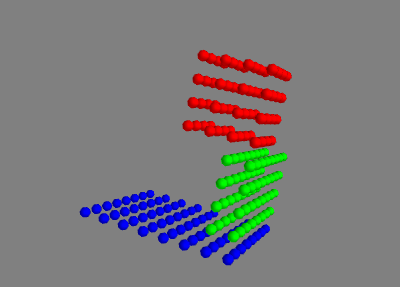
\includegraphics[width=0.48\textwidth]{Pic/allocationshape/allocation}
  \caption{64-node job with different allocation shapes. Red, Green and Blue represents 3D balance, 3D unbalance and 2D balance allocation respectively. }
  \label{fig: allocation}
\end{figure}

The workload traces we used for evaluating our new scheduling framework consist of jobs with size variation from 64 to 16K. Due to space limitation, we only present the results for job size 64 and 512, both conforms to three different communication patterns. We suppose the scale of the torus network simulated in this experiment is set to $32 \times 32 \times 32 $, $32,768$ nodes in total, thus all the possible allocation for job with size 64 and 1024 are shown in table \ref{table:allocationvector}. Since we construct a symmetric 3D torus network in our simulation (the bandwidth of each link in x, y, x direction are the same), we suppose the allocation with $v=\{x, y, z\}$ is the same compared to all the other allocations with the dimension of the permutation of \{x, y, z\} in terms of jobs performance.

\begin{table}
\caption{Different allocation vectors for job with size 64-node and 512-node}
\label{table:allocationvector}
\begin{center}
\begin{tabular}{llllr}
\toprule
\multicolumn{4}{c}{Item} \\
\cmidrule(r){2-5}
Job Size    & 3D-B & 3D-UB & 2D-B & 2D-UB  \\
\midrule
64-node      & \{4,4,4\}    & \{8,4,2\}   & \{8,8,1\}  & \{16,4,1\}      \\
             &       &     &      & \{32,2,1\} \\
\midrule
512-node    & \{8,8,8\}   & \{16,8,4\} &     &       \\
            &       & \{16,16,2\} &    &  \{32,16,1\}      \\
            &  & \{32,8,2\} & &\\
            &  & \{32,4,4\} & &\\
\midrule
1024-node    &    & \{16,8,8\} &   \{32,32,1\}  &       \\
            &       & \{16,16,4\} &    &       \\
            &  & \{32,8,4\} & &\\
            &  & \{32,16,2\} & &\\
            
 \bottomrule
\end{tabular}
\end{center}
\end{table}




In our simulation, we set the packet size $\delta$ to 256 Byte. The amount of data transferred by each node pair $m_{i,j}$ is set to 2KB, which indicates $2KB/256B = 8$ packets will be transfterred between each node pair through the job's execution. The number of packets transferred between each node pair $\sigma = m_{i,j}/\delta$. The job size in the simulation is set to $n$.

\begin{table}
\caption{Nomenclature}
\label{table:nomenclature}
\begin{center}
  \begin{tabular}{ l | c }
    \hline \hline
    Symbol 	& Description \\ \hline \hline
    $\delta$ 	& packet size. \\ \hline
    $\sigma$    & the number of packets transferred between each node pair. \\ \hline
    $\Delta$    & the total amount of data generated by each node, $\Delta = \delta \cdot \sigma$. \\ \hline
    $N $   	& System size, i.e., the number of nodes in the system.\\ \hline
    $n$    & job size, i.e., the number of nodes required by the job.\\ \hline
    $M$    & the communication pattern matrix of each job.\\ \hline
    $m_{i,j}$ 	& the amount of data transferred between process $p_i$ and $p_j$. \\ \hline
    $D$    & the distance matrix of the allocation of each job. \\ \hline
    $d_{i,j}$    & the distance between node $i$ and $j$. \\ \hline
    \hline
  \end{tabular}
\end{center}
\end{table}

\subsection{Results}
\label{sec:results}
Given the system is $32\times 32 \times 32$ symmetric 3D torus, table \ref{table:allocationvector} shows all the possible allocation vectors for jobs with 64/512-node. Table \ref{tab: 64/512node-job} shows the normalized runtime of these two jobs conform to four different communication patterns with each allocation vector. As shown in table \ref{table:allocationvector}, there could be multiple allocation vectors for the same shape, such as the 512-node job could have 4 different allocation vectors with 3D unbalance shape. The average value of differnt allocation vectors for the same shape is presented in table \ref{tab: 64/512node-job}.

\begin{table}[ht]
\begin{center}
\caption{job conforms to four different communication patterns running 3D torus system. In each row, the values on the upper level are the results for 64-node job, the lower level are for 512-node job.
\textcolor{red}{Results in this table would be provided by CODES simulation, job scale depends on the job traces we decide to use}} 
\label{tab: 64/512node-job}
\begin{tabular}{l c c c c c} 
\toprule % Top horizontal line
\toprule
&\multicolumn{5}{c}{Allocation} \\
\cmidrule(l){2-6}
Communication Pattern $M$ & 3D-B & 3D-UB & 2D-B & 2D-UB & NC \\ % Column names row

\midrule % In-table horizontal line
$M_{a2a}$   & 1  &   &    &   &  \\ % Content row 1
           & 1  &   &    &   &  \\ % Content row 1
\midrule
$M_{nn}$  & 1  &   &    &   &  \\ % Content row 1
            & 1  &   &    &   &   \\ % Content row 1
\midrule
$M_{o2a}$   & 1  &   &    &   &  \\ % Content row 1
            & 1  &   &    &   & \\ % Content row 1
\midrule
$M_{a2o}$    & 1  &   &    &   & \\ % Content row 1
             & 1  &   &    &   &  \\ % Content row 1
% \midrule
% $M_{hyb}$   & 1 & 1.24 & 1.37  & 1.66 \\ % Content row 1
%             &  &  &    \\ % Content row 1
\midrule
\bottomrule % Bottom horizontal line
\end{tabular}
\end{center}
\end{table}



\section{Scheduling Mechanism}
\label{sec:scheduling mechanism}

Figure \ref{fig:overall design} shows the overall design of our new scheduling framework. It takes not only job size, user estimated runtime, but also job's communication pattern (CP) as input parameters. The CP here is provided by user, which indicate the most dominant communication pattern of the user job, such as All-to-All, Nearest Neighbor, Collective, ect. The detailed amount of communication data is neither necessary nor possible in this communication pattern. As we prove in section \ref{sec:communication pattern matrix}, job with different CP has different preference about network requirement, hence different preference about allocations. For example, job with All-to-All communication pattern requires more network resource, which means a compact or torus allcoation will guarantee a better performance. However, job conforms to Nearest Neighbor communication pattern won't fully utilize the torus network or compact allocation, which means a mesh allocation will serve it equally well.


\begin{figure}[h!]     
\centering  
\includegraphics[width=0.48\textwidth]{Pic/design/overalldesign}  
\caption{Overview of our new scheduling framework. It takes not only job size, user estimated runtime, but also job's communication pattern matrix as input and combines these user provide information with system information to make optimal prioritizing and allocation decisions. It also maintains hashtable, which provides quick reference for making the specific allocation for incoming job with distinct communication pattern. }
\label{fig:overall design}
\end{figure}


Since HPC workload tend to be repetive, our new scheduling framework keep record of historic jobs information to provide quick reference for making the preferable allocation for incoming job with distinct communication pattern. When user submit his job, our new scheduler will first look for job's user name and executable file name in historic record to check whether this job been submitted before. Then the scheduler gets the job's input parameter \{S, CP, ERT\} (job size, Expected RunTime, CommunicationPattern),  and check in the historic data to identify its preferred allocation. As time goes by, our new framework will gradually build up a comprehensive record of all the possible job submission, which is helpful to provide quick reference for the future jobs. Due to the repetitiveness of the workload, the size of this record will grows rapidly at first, then gently grow for a while and come to stagnation, as shown in figure
\ref{fig:table size growth}. 

\begin{figure}[h!]     
\centering  
\includegraphics[width=0.48\textwidth]{Pic/design/tablesize}  
\caption{The size growth of historic submitted job records.}
\label{fig:table size growth}
\end{figure}


 We implement a record mechanism as the central component in our framework to keep track of the pattern in workload repetitiveness, hence make predictive optimizations in terms of both job and system performance. Firgure \ref{fig:scheduling mechanism} shows the overview of our design. The scheduler start to build the table since the first submitted job. When user submit a job, the scheduler get job's size and communication pattern, then check the record to find the best allocation for the job. On the other hand, the available resource will be categorized and organized into different types, such as 3D balance, 3D unbalance, 2D balance, 2D unbalance (toruse or mesh). All these available resource will be updated with real-time system feedback information. When a job is finished, the resource it released can be merge into the neighboring one (if the neighbor is also available) to come up with a bigger chunk. So the 2D resource can become into 3D by merging with newly released ones, so does mesh to torus.

\begin{figure}[h!]     
\centering  
\includegraphics[width=0.48\textwidth]{Pic/design/referencetable}  
\caption{overview of scheduling mechanism}
\label{fig:scheduling mechanism}
\end{figure}

With the feedback from system, our scheduling framework will become knowledgeable about the preference of jobs with different communication pattern. The feedback information keep the batch scheduler updated with the latest status of the system such as the number of available nodes, their layout and geometry,  when hotspot or bottleneck come up in network, etc. The scheduler schedule/dispatch the following jobs adaptively based these information.


Our new scheduling framework is designed based on the knowledge about the precognition of workload. The scheduler works periodically and take 3 steps in each scheduling cycle. The scheduling cycle can be predefined by a fixed time interval, or triggered by events like job completion. The 3 steps within each scheduling cycle are

\begin{itemize}

    \item \textbf{Update resource lists from system feedback}. The resource management module take the feedback information form system and refresh the resource lists every time there is a job completes. The resource released by the job can be merged with any other available resource adjacent to it, in order to form up more compact resources. This is similar to Garbage Collection mechanism in memory management. 1D or 2D resource can become 3D resource and unbalance resource become balance resource after being merged with others. The resource list is well organized when the update is finished, thus, better job scheduling 
    
    \item \textbf{Job prioritization and allocation}. With job's information like size, expected runtime, dominant communication pattern provided upon submission and the well organized resource list maintained by resource management module, our scheduler will make decision about timing and location of each job being dispatched to the system. The scheduling policy will be discussed in detail in \ref{sec:scheduling policy}.

    
    \item \textbf{Update reservation}. When a job couldn't get its optimal reousrce allocation and any available suboptimal allocation can not compensate the job's performance lose, the job has an option to make reservation for its optimal resource. Therefore, each time a job got dispatched, the scheduler need to update the reservation, delete those that been satisfied and reserve for the following jobs if necessary.


\end{itemize}



\section{Scheduling Policy}
\label{sec:scheduling policy}

We designed and implemented two scheduling algorithms, Rackless and Cautious, for our new scheduler framework. Both of them take advantage of the scheduler's workload precongnition ability and can deliver comparable performance improvement 
as against the traditional schedulers. The comparision results are presented in \ref{sec:scheduling results}.


Before we introduce our scheduling policy, we will first give explanation about workload and system. Suppose the system has 3D torus network and the available resource is consist of a set of 3D or 2D sub-torus chunks, which can be denoted by $\{v\}$, each $v_i = \{x_i, y_i, z_i\}$. The size of each chunk $v_i$, $S_{v_i} = x_i\cdot y_i\cdot z_i $. 

The job set in the scheduling window is denoted by $\{J\}$, each $J_i$ has size $S_{J_i}$. Due to the repetitiveness of the workload, $S_{J_i} \in \{n_1, n_2, .., n_k\}$, where $k \leq 5$. 
We can make two reasonable assumption about $\{v\}$ and $\{J\}$. 

\begin{equation}
\label{eq:mod0}
\exists S_{v_i} > S_{v_j} \quad then\quad S_{v_i} \bmod S_{v_j} \equiv 0
\end{equation}


\begin{equation}
\label{eq:nofrag}
\min S_{J_i} \leq \min S_{v_i} 
\end{equation}

The reason for both Equation \ref{eq:mod0} and \ref{eq:nofrag} stand is the repetitiveness of workload.

\subsection{Scheduling Policy 1: Reckless}
\label{sec:reckless}

Reckless is designed to be responsive. The overhead for Reckless to make scheduling decision is very low, such that it can be competent when system has high job arrival rate. Reckless first pick a job from the scheduling window and check according the job's size and communication pattern if its optimal resource is availbale. The job get run when enough optimal resource is available. However, if there is no enough optimal resource and only enough sub-optimal availale, Reckless will make reservation if job with ATA communication pattern and run job with non-ATA communication pattern anyway. And if there is no enough resource for any job in the scheduling window, Reckless will hold and skip the current scheduling cycle, wait for more resource got released and make scheduling in the next cycle.

\begin{algorithm}
  \label{alg:scheudling1}
  \caption{Reckless}
  \begin{algorithmic}
    \State \{J\}, Job set in the scheudling window
    \State \{v\}, available system resource sets
    \While{\{J\} is not empty}
        
        \If{optimal $v_i$ is available for $j_i$}
            \State run $j_i$ on $v_i$;
            \State delete $j_i$ from \{J\};
            \State update reservation;
        \EndIf
        
        \If{$\exists \bar{v_i}$ satisfy $j_i$ AND $\bar{v_i}$ is not optimal}
            \If{$j_i$ is ATA dominant}
                \State Wait and Reserve $\hat{v_i}$;
            \EndIf
            \If{$j_i$ is not ATA dominant}
                \State run $j_i$ on $\bar{v_i}$;
                \State delete $j_i$ from \{J\};
                \State update reservation;
            \EndIf
        \EndIf
        
        \If{Available \{$v_i$\} $leq$ $forall$$j_i$ requirement}
            \State hold;
        \EndIf
        
    \EndWhile
  \end{algorithmic}
\end{algorithm}


\subsection{Scheduling Policy 2: Cautious}
\label{sec:cautious}

Our second scheduling algorithm named Cautious. The difference between Reckless and Cautious is that, Cautious always make evaluation before it assign job to sub-optimal resources. The most intuitive evaluation metric is job's turn-around time. As shown in \ref{alg: Evaluate}, it will compare the runtime for job on the sub-optimal resource, and the time for waiting optimal resource plus the runtime for job on optimal resource. The result will decide whether the job will run on the sub-optimal resource promptly or wait and reserve for its optimal resource.

The other evaluation metrics for Cautious to make decision in terms of system is the Lose of Capacity(LOC). As we shown before, the optimal resource always requires embazzle more network resource, which further leads to system fragmentation, and thus low system utilization. The system administrator is free to choose the evaluation metrics here based on the system and workload features.


\begin{algorithm}
  \label{alg:scheudling2}
  \caption{Cautious}
  \begin{algorithmic}
    \State \{J\}, Job set in the scheudling window
    \State \{v\}, available system resource sets
    \While{\{J\} is not empty}
           
        \If{optimal $v_i$ is available for $j_i$}
            \State run $j_i$ on $v_i$;
            \State delete $j_i$ from \{J\};
            \State update reservation;
        \EndIf
        
        \If{$\exists \bar{v_i}$ satisfy $j_i$ AND $\bar{v_i}$ is not optimal}
            \If{Evaluate($j_i$, $\bar{v_i}$)}
                \State run $j_i$ on $\bar{v_i}$;
                \State delete $j_i$ from \{J\};
                \State update reservation;
            \Else
                \State Wait and Reserve $\hat{v_i}$;
                \State Choose from \{J\}-$j_i$ do Backfilling;
            \EndIf
        \EndIf
        
        \If{Available \{$v_i$\} $\leq$ $\forall$$j_i$ requirement}
            \State hold;
        \EndIf
        
    \EndWhile
    
  \end{algorithmic}
\end{algorithm}



\begin{algorithm}
  \label {alg: Evaluate}
  \caption{Evaluate($j_i$, $\bar{v_i}$)}
  \begin{algorithmic}
    \State Get $\bar{t}$, the time for job $j_i$ to complete on suboptimal resource $\bar{v_i}$;
    \State Get $\hat{t}$, the time for job $j_i$ to complete on optimal resource $\hat{v_i}$;
    \State Get $\delta{t}$, the time job $j_i$ wait for optimal resource $\hat{v_i}$;
    \If{$\delta{t} + \hat{t} \leq \bar{t}$}
        \State return False;
    \Else
        \State return True;
    \EndIf
    
  \end{algorithmic}
\end{algorithm}

Both Reckless and Cautious has its pros and cons. Reckless is responsive and efficient, but it make scheduling decision lack of thoughts. The job may suffer a long run time when it assign to sub-optimal resource and can lead to potential system fragmentation. Cautious, on the other hand, spends time for evaluation if there is only sub-optimal resource for the job. 



\section{Evaluation Methodology}
\label{sec: evaluation methodology}

We conduct a series of experiments using the traces described in Section \ref{sec:job traces} to evaluate our design as against two most frequently used scheduling/allocation policies. Both of them use FCFS/EASY backfilling for job prioritizing. When it comes to job allocation, the first use contiguous/compact allocation strategy (\textbf{CC}), which means the nodes within the allocation it assigned to every job are spacially contiguous and compact. The partition-based allocation strategy used in IBM Blue Gene series of machines are of this kind. The second use non-contiguous allocation strategy(\textbf{NC}), which means it provide jobs with allocation without consideration about the adjacency of nodes. The nodes within each allocation could be scattered all over the system. Machines from Cray Inc. use similar allocation strategy like \textbf{NC}. Both the traditional \textbf{NC} and \textbf{CC} are agnostic about workload. In the rest of the paper, we use \emph{Reckless}, \emph{Cautious}, \emph{CC} and \emph{NC} to denote our scheduling policies and the default ones.

\subsection{Evaluation Metrics} 
\label{sec:metrics}
We use three scheduling metrics for the evaluation of our scheduling framework as against the default ones. They have been chosen for the quantified analysis of both system and job's performance.

\begin{itemize}
  
  \item \emph{System Utilization Rate}.  System Utilization Rate can be calculated in the following way. Suppose $T$ is the total elapsed time for $J$ jobs, $t_e$  the completion time for job $i$ and $t_s$ be its the start time, and $n_i$ be the size of job $i$, then system utilization rate is calculated as
  
  \begin{eqnarray}\displaystyle
  \dfrac{\sum_{0\leq i\leq J}{(t_e-t_s) \cdot n_i}}{N \cdot T}
  \end{eqnarray} 
  
  \item \emph{Average Wait Time}. For each job, its wait time refers to the time elapsed between the moment it is submitted and the moment it is dispatched to run. This metric is calculated as the average across all the jobs submitted to the system. The batch scheduler should cut job's wait time down as much as possible.
  
   \begin{eqnarray}\displaystyle
    T_{wait} = t_{start}-t_{arrive}
  \end{eqnarray} 
  
  
	\item \emph{Average Job Response time}. Response time refers to the amount of time it take when each job is submitted until it ends, which equals to its wait time plus its run time.
       
  \begin{eqnarray}\displaystyle
    T_{response} = T_{run}+T_{wait}
  \end{eqnarray}   
	
\end{itemize}

A good batch scheduler should always balance system's performance and user job's performance. On one hand, the batch scheduler should be as responsive as possible, so that user job won't wait too long to get served. On the other hand, the batch scheduler should always guarantee a relative high and stable system uilization so that system resource can be fully utilized.


\subsection{CQSim: Trace-based Scheduling Simulator}
%\textbf{\textcolor{red}{This subsection is Self Plagiarized from Cluster14!!!!}}\\

Simulation is an integral part of our evaluation of various allocation policies
as well as their aggregate effects on system utilization, job's wait time and
response time. We have developed a simulator named CQSim to evaluate our design
at scale. The simulator is written in Python, and is formed by several modules
such as job module, node module, scheduling policy module, etc. Each module is
implemented as a class. The design principles are reusability, extensibility,
and efficiency. The simulator takes job events from the trace, and an event could be
job submission, start, end, and other events. Based on these events, the
simulator emulates job submission, allocation, and execution based on specific
scheduling and allocation policies. CQsim is open source, and is available to the
community \cite{Cqsim}.  \\



\subsection{Job Traces}
\label{sec:job traces}
%\textbf{\textcolor{red}{This subsection is Self Plagiarized from Cluster14!!!!}}\\

In this work, we use two real workload traces collected from production
supercomputers to evaluate our design. The objective of using multiple traces is
to quantify the performance of our design when dealing jobs and systems with
different characteristics. The first trace we used is from a machine named Blue Horizon at
the San Diego Supercomputer Center (denoted as SDSC-BLUE in the paper), which
contains 4,830 jobs. The second trace we used is from a IBM Blue Gene/P system
named Intrepid at Argonne National Laboratory (denoted as ANL-Intrepid in the paper)
\cite{par}. This trace contains 2,612 jobs. Figure \ref{fig:jobsizeintowtraces}
summarizes job size distribution of these traces. ANL-Intrepid is used to
represent capability computing where jobs require a large amount of computing
nodes for solving large-scale problems, whereas SDSC-BLUE is used to represent
capacity computing where the system is utilized to solve a large number of
small-sized problems.

\begin{figure}[h!] 
  \centering
  \includegraphics[width=0.38\textwidth]{Pic/JobInfo/job_dist}
   \caption{Job size distribution of ANL-Intrepid and SDSC-BLUE }
   \label{fig:jobsizeintowtraces}
\end{figure}


\section{Experiment Results}
\label{sec:scheduling results}

\textcolor{red}{all the figs in this section are obsolete!!!}

\begin{figure}[h!] 
  \centering
  \includegraphics[width=0.48\textwidth]{Pic/experiment/summary/utilization}
  \caption{System Utilization got from CC, NC, Greedy, Cautious respectively}
  \label{fig: uti}
\end{figure}


\begin{figure}[h!] 
  \centering
  \includegraphics[width=0.48\textwidth]{Pic/experiment/summary/awt-vs-cc}
  \caption{Jobs' average wait time reduction got by comparing CC as against our design.}
  \label{fig: uti}
\end{figure}


\begin{figure}[h!] 
  \centering
  \includegraphics[width=0.48\textwidth]{Pic/experiment/summary/art-vs-cc}
  \caption{Jobs' average response time reduction got by comparing CC as against our design.}
  \label{fig: uti}
\end{figure}

\begin{figure}[h!] 
  \centering
  \includegraphics[width=0.48\textwidth]{Pic/experiment/summary/awt-vs-nc}
  \caption{Jobs' average wait time reduction got by comparing NC as against our design.}
  \label{fig: uti}
\end{figure}


\begin{figure}[h!] 
  \centering
  \includegraphics[width=0.48\textwidth]{Pic/experiment/summary/art-vs-nc}
  \caption{Jobs' average response time reduction got by comparing NC as against our design.}
  \label{fig: uti}
\end{figure}



\section{Related Work}
\label{sec:related_work}
Batch scheduling on HPC system has been a hot topic getting constant discussion since the 1990's.
Feitelson et al proposed the most widely used job scheduling policy which is First Come, First Serve (FCFS) combined with 
EASY backfilling\cite{feit}. FCFS/EASY backfilling policy greatly improves HPC system's utilization and cuts the wait time 
of first job in the waiting queue. Since then, many studies seek to refine this classic scheduling paradigm. Tang et al. 
tried to improve the accuracy of user's estimated job runtime and walltime so as to enhance the efficiency of backfilling and  minimize the system fragmentation\cite{wei-ipdps2010} \cite{wei-jpdc2013} \cite{wei-ipdps2011}. % And there are some other variation of FCFS/EASY backfilling proposed to optimize system performance in terms of power consumption and energy cost \cite{zhou}\cite{yang-sc13}.


Only with the information about job size and estimated run time seems to be insufficient for batch scheduler do make the 
optimal scheduling/allocaiton decision. Some work proposed that the batch scheduler should be aware of some information 
about system network information in order to fully utilize system resources.Leung et al. presented allocation strategies 
based on space filling curves and one dimensional packing \cite{leung}. The problem with using space filling curve is that  
it can only be applied to system with the scale of $2^n$ nodes in each dimension, which is a ideal case that not existing 
in morden HPC systems. Albing et al. conducted study about the allocation strategies that the Cray
Application Level Placement Scheduler (ALPS) used \cite{carl-cug}. The job allocation in Cray Linux Environment (CLE) 
operating system is managed by ALPS, which simply works off an ordered node list, however that is ordered. 

Based on their 
work, Yang et al. presented a window-based locality-aware job scheduling design for torus-connected system
\cite{yang-cluster14}. In this new scheduling framework, several jobs are taken into  consideration at the same time for job 
prioritizing and resource allocation. A list of slots is maintained to preserve node contiguity information for
resource allocation. Each job been assigned into one of these slot so that the locality can be mostly preserved.

Rosenthal et al. found there is limited benefit for many applications by
increasing network bandwidth \cite{rosenthal}. They employed a subset of the
CORAL mini-applications that represent U.S. Department of Energy workload and
leverage multirail networkings to evaluate the improvement of these applications
caused by increased network bandwidth. The applications that send mostly small
messages or larger messages asynchronously are not bandwidth bounded, hence,
benefit only slightly or not at all from increased bandwidth.

   

Hoefler et al. propose to use performance modeling techniques to analysis 
factors that impact the performance of parallel scientific applications 
\cite{hoefler-modeling}. However, as the scale of HPC continue grows, the 
interference of concurrently running jobs is getting worse, which is hard to be 
quantified by performance profiling tools.


Bogdan et al provide a set of guidelines how to configure a network with 
Dragonfly topology for workload with Nearest Neighbor communication 
pattern\cite{Bogdan-hpdc14}. They first derived a theoretical model of Nearest 
Neighbor communication performance on Dragonfly network that can predict network 
bottleneck. Then, they use simulation to validate the correctness of their 
theoretical model.

Dong et al describe IBM Blue Gene/Q's 5D torus interconnect
network\cite{Dong-SC11}. They developed simple benchmarks that conforms to four
different communication patterns, namely ping-pong, nearest neighbor, broadcast
and allredcue, to demonstrate the effectiveness of this highly parallel 5D torus
network.



\section{Conclusions}
\label{sec:conclusion}


\section*{Acknowledgment}
\label{sec: ack}
%We appreciate the valuable comments and suggestions from the anonymous reviewers. 
The work at Illinois Institute of Technology is supported in part by
US National Science Foundation grant CNS-1320125. The work at Argonne is
supported in part by the U.S. Department of Energy (DOE), Office of Science,
under Contract DE-AC02-06CH11357.



\begin{thebibliography}{10}
 %=====start of scheduling papers===== 
\bibitem{feit}
D.~Feitelson and A.~Weil.
\newblock Utilization and predictability in scheduling the {IBM} {SP2} with
  backfilling.
\newblock In {\em International Parallel and Distributed Processing Symposium}, 1998.

\bibitem{wei-ipdps2010}
W.~Tang, N.~Desai, D.~Buettner, and Z.~Lan.
\newblock Analyzing and adjusting user runtime estimates to improve job
  scheduling on the {Blue} {Gene/P}.
\newblock In {\em 2010 IEEE International Symposium on Parallel Distributed
  Processing}, 2010.

\bibitem{wei-ipdps2011}
W.~Tang, Z.~Lan, N.~Desai, D.~Buettner, and Y.~Yu.
\newblock Reducing fragmentation on torus-connected supercomputers.
\newblock In {\em 2011 IEEE International Symposium on Parallel Distributed
  Processing Symposium}, 2011.

\bibitem{wei-jpdc2013}
W.~Tang, N.~Desai, D.~Buettner, and Z.~Lan. 
\newblock Job Scheduling With Adjusted Runtime Estimates on Production Supercomputers.
\newblock Journal of Parallel and Distributed Computing (JPDC), 73(7):926-938, 2013.

\bibitem{zhou}
Z.~Zhou, Z.~Lan, W.~Tang, and N.~Desai.
\newblock Reducing energy costs for {IBM Blue} {Gene/P} via {Power-Aware} job
  scheduling.
\newblock In {\em 17th Workshop on Job Scheduling Strategies for Parallel
  Processing}, 2013.

\bibitem{yang-sc13}
X. ~Yang, Z.~Zhou, S.~Wallace Z.~Lan, W.~Tang, S. ~Coghlan and Mike. ~Papka.
\newblock Integrating Dynamic Pricing of Electricity into Energy Aware Scheduling for HPC Systems. 
\newblock In {Proceedings of the International Conference on High Performance Computing, Networking, Storage and Analysis(SC), 2013 International Conference for}
\newblock SC '13,
\newblock 2013,
\newblock Salt Lake City, Utah

\bibitem{Cqsim}
{\textcolor{red} {Cqsim: An event-driven simulator}}.
\newblock http://bluesky.cs.iit.edu/cqsim


%=====start of allocation aware papers===== 
\bibitem{leung}
Leung, V.J.; Arkin, E.M.; Bender, M.A.; Bunde, D.; Johnston, J.; 
Alok Lal; Mitchell, J.S.B.; Phillips, C.; Seiden, S.S., 
\newblock Processor allocation on Cplant: achieving general processor locality using one-dimensional allocation strategies
\newblock In {Proceedings of 2002 IEEE International Conference on Cluster Computing, 2002}.  pages 296--304, 2002

\bibitem{carl-cug}
Carl Albing and Mark Baker
\newblock ALPS,Topology, and Performance: A Comparison of Linear Orderings for 
Application Placement in a 3D torus.
\newblock Presented at the CUG 2010, Edinburgh, Scotland, UK, 2010.

\bibitem{yang-cluster14}
Xu Yang and Zhou Zhou and Wei Tang and Xingwu Zheng and Jia Wang and Zhiling Lan.
\newblock Cluster Computing (CLUSTER), 2014 IEEE International Conference on,
\newblock Balancing job performance with system performance via locality-aware scheduling on torus-connected systems
\newblock Sept, 2014,
\newblock pp.140-148

%+++++++++++++++++++++++
\bibitem{mpip}
\newblock mpiP: Lightweight, Scalable MPI Profiling.
\newblock http://mpip.sourceforge.net, 
\newblock 2013.

\bibitem{tau}
S. Shende and A. Malony. 
\newblock The TAU parallel performance system. 
\newblock International Journal of High Performance Computing Applications, 20(2):287–311, 2006.

\bibitem{scala}
X. Wu, F. Mueller, S. Pakin, 
\newblock "Automatic Generation of Executable Communication Specifications from Parallel Applications", 
\newblock In {Proceedings of the International Conference on High Performance Computing, Networking, Storage and Analysis(SC), 2011 International Conference for}
\newblock SC '11,
\newblock 2011,pages 12-21.

%+++++++++++++++++

%=====start of network papers===== 
\bibitem{rosenthal}
E. Rosenthal and E.A. Leon
\newblock Characterizing Application Sensitivity to Network Performance.
\newblock  In {Proceedings of SC14: International
Conference for High Performance Computing, Networking, Storage and Analysis},
2014

\bibitem{hoefler-modeling}
T. Hoefler and W. Gropp and M. Snir and W. Kramer
\newblock Performance Modeling for Systematic Performance Tuning,
\newblock 2011
\newblock Nov.
\newblock In {Proceedings of International Conference for High Performance Computing, Networking, Storage and Analysis (SC'11), SotP Session,
}

\bibitem{roth}
P. Roth and J. Meredith and J. Vetter,
\newblock "Automated Characterization of Parallel Application Communication Patterns",
In Proceedings of the 25rd International Symposium on High-performance Parallel and Distributed Computing
\newblock HPDC '15,
\newblock 2015,


%=====end of application/mapping papers===== 
\bibitem{Pjesivac}
Pje\v{s}ivac-Grbovi\'{c}, Jelena and Angskun, Thara and Bosilca, George and Fagg, Graham E. and Gabriel, Edgar and Dongarra, Jack J.
\newblock Performance Analysis of MPI Collective Operations,
\newblock Cluster Computing,
\newblock June 2007,
\newblock volume 10,
\newblock numpages 17,
 

\bibitem{thakur}
Thakur, Rajeev and Gropp, William D.
\newblock Improving the performance of collective operations in MPICH,
\newblock Recent Advances in Parallel Virtual Machine and Message Passing Interface,
\newblock year 2003,
\newblock Springer

\bibitem{abhinav-ipdps15}
Abhinav Bhatele, Andrew R. Titus, Jayaraman J. Thiagarajan, Nikhil Jain, Todd Gamblin,
Peer-Timo Bremer, Martin Schulz† and Laxmikant V. Kale,
\newblock "Identifying the Culprits behind Network Congestion",
\newblock In {\em 2015 IEEE International Symposium on Parallel Distributed Processing Symposium}, 2015.

\bibitem{langer}
S. Langer, A. Bhatele, and C. H. Still,
\newblock “pF3D simulations of laser-plasma interactions in National Ignition Facility experiments,” 
\newblock Computing in Science and Engineering, vol. 99, Aug. 2014, lLNL- JRNL-648736. 
\newblock [Online]. Available: http://doi.ieeecomputersociety.org/ 10.1109/MCSE.2014.79

%\bibitem{abhatele-ipdps08}
%A. Bhatele, L.V.  Kale
%\newblock Application-specific topology-aware mapping for three dimensional topologies.
%\newblock In {\em Proceedings of Workshop on Large-Scale Parallel Processing (held as part of IPDPS' 08)} 2008
%
%\bibitem{abhinav-sc13} 
%Bhatele, Abhinav and Mohror, Kathryn and Langer, Steven
%H. and Isaacs, Katherine E. 
%\newblock There Goes the Neighborhood: Performance Degradation Due to Nearby Jobs 
%\newblock In {Proceedings of SC13: International
%Conference for High Performance Computing, Networking, Storage and Analysis},
%2013

\bibitem{hpdc14}
Prisacari, Bogdan and Rodriguez, German and Heidelberger, Philip and Chen, Dong and Minkenberg, Cyriel and Hoefler, Torsten
\newblock Efficient Task Placement and Routing of Nearest Neighbor Exchanges in Dragonfly Networks
\newblock In Proceedings of the 23rd International Symposium on High-performance Parallel and Distributed Computing
\newblock HPDC '14,
\newblock 2014,
\newblock Vancouver, BC, Canada

\bibitem{jingjin}
Wu, Jingjin and Lan, Zhiling and Xiong, Xuanxing and Gnedin, Nickolay Y. and Kravtsov, Andrey V.
\newblock Hierarchical Task Mapping of Cell-based AMR Cosmology Simulations
\newblock Proceedings of the International Conference on High Performance Computing, Networking, Storage and Analysis
\newblock SC '12,
\newblock 2012,
\newblock Salt Lake City, Utah

\bibitem{zhou-ipdps}
Z. Zhou, X. Yang, Z. Lan, P. Rich, W. Tang, V. Morozov, and N. Desai.
\newblock Improving Batch Scheduling on Blue Gene/Q by Relaxing 5D Torus Network Allocation Constraints,
\newblock Proceedings of 29th IEEE International Parallel \& Distributed Processing 
Symposium,
\newblock IPDPS'15, 2015.
\newblock Hyderabad, INDIA

\bibitem{Bogdan-hpdc14}
Prisacari, Bogdan and Rodriguez, German and Heidelberger, Philip and Chen, Dong and Minkenberg, Cyriel and Hoefler, Torsten
\newblock Efficient Task Placement and Routing of Nearest Neighbor Exchanges in Dragonfly Networks,
\newblock Proceedings of the 23rd International Symposium on High-performance Parallel and Distributed Computing,
\newblock HPDC '14,
\newblock 2014,
\newblock  Vancouver, BC, Canada,

\bibitem{Dong-SC11}
Dong Chen; Eisley, N.A.; Heidelberger, P.; Senger, R.M.; Sugawara, Y.; Kumar,
S.; Salapura, V.; Satterfield, D.L.; Steinmacher-Burow, B.; Parker, J.J., 
\newblock "The IBM Blue Gene/Q interconnection network and message unit," 
\newblock High Performance Computing, Networking, Storage and Analysis (SC), 2011 International 
Conference,
\newblock pp.1,10, 
\newblock 12-18 Nov. 2011

\bibitem{Jason-2011}
Jason Cope, Ning Liu, Sam Lang, Phil Carns, Chris Carothers, Robert Ross.
\newblock Proceedings of the Workshop on Emerging Supercomputing Technologies 2011,
\newblock 2011


%===simulation papers =====

\bibitem{ross}
C. Carothers, D. Bauer, and S. Pearce.
\newblock ROSS: A High-Performance, Low memory, Modular Time Warp System. 
\newblock Journal of Parallel and Distributed Computing,
\newblock (62):1648–1669, 2002.

\bibitem{mubarak-sc2012}
Mubarak, M.; Carothers, C.D.; Ross, R.; Carns, P.,
\newblock "Modeling a Million-Node Dragonfly Network Using Massively Parallel Discrete-Event Simulation," 
\newblock High Performance Computing, Networking, Storage and Analysis (SCC), 
\newblock 2012 SC Companion: 
\newblock pp.366,376, 10-16 Nov. 2012




\end{thebibliography}

\end{document}


